

\section{Introduction}

\begin{frame}

    \frametitle{The Opioid Crisis} % Title
    \framesubtitle{}  % Subtitle
    \rmfamily % Font

    \begin{wideitemize}
        \item 110,000 Americans died in 2022 as a consequence of drug abuse
    \end{wideitemize}

    \begin{center}
        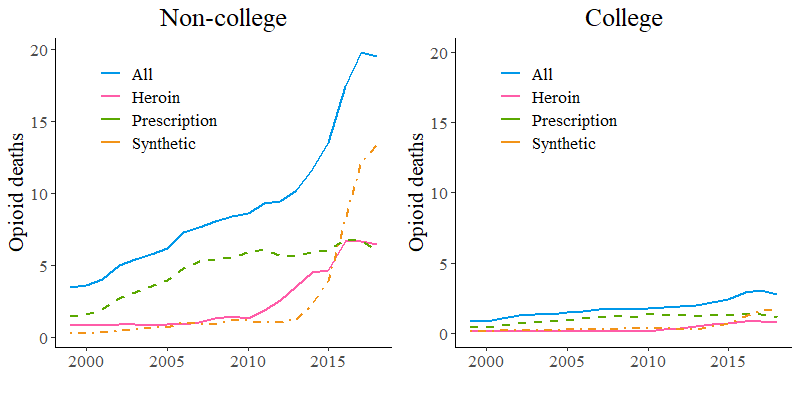
\includegraphics[scale=0.5]{ODD.png}
    \end{center}

    {\footnotesize \textit{Opioid deaths for both the non-college and college-educated as measured per 100,000 people in the respective education class (\textcolor{fgre}{Greenwood, Guner and Kopecky, 2022})}}
    
\end{frame}


\begin{frame}

    \label{Minimum Wage}
    \frametitle{State minimum wage trends} % Title
    \framesubtitle{}  % Subtitle
    \rmfamily % Font
    
    \begin{wideitemize} 
        \item States have been increasing their \textcolor{fblu}{minimum wage rates}, with varying intensity
    \end{wideitemize}

    \begin{center}
        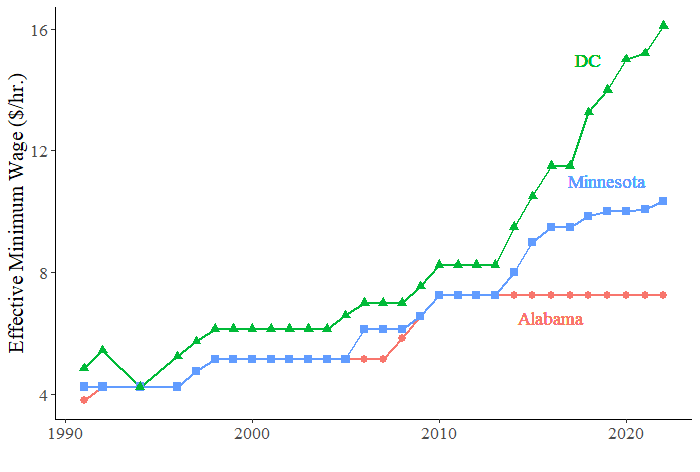
\includegraphics[scale=0.5]{min_wage_plot_simp.png}
    \end{center}
    
    \hyperlink{min_wage_plot_allstates}{\beamerbutton{All states}}
    
\end{frame}


\begin{frame}

    \frametitle{Main idea} % Title
    \framesubtitle{}  % Subtitle
    \rmfamily % Font
    
    \begin{wideitemize}
        \item Opioid misuse can lead the victims to negative labor market outcomes
        \item Minimum wage rates affect these outcomes 
        \vspace{9pt}
        \begin{wideitemize}
            \item[\textcolor{fblu}{\textbullet}] Negatively, through their impact on \textcolor{fblu}{labor demand for low-skill jobs} 
            \item[\textcolor{fblu}{\textbullet}] Positively, if they address the reasons that cause \textcolor{fblu}{addiction} in the first place \(\to\) \textcolor{fblu}{Deaths of despair}
        \end{wideitemize}
        \item The dominance of each effect depends on how \textcolor{fblu}{binding} minimum wage rates are across labor markets
    \end{wideitemize}

\end{frame}


\begin{frame}

    \frametitle{In this paper I ask} % Title
    \framesubtitle{}  % Subtitle
    \rmfamily % Font
    
    \begin{wideitemize}
        \item Do the effects of \textcolor{fblu}{Opioid Use Disorders} (\textcolor{fblu}{OUDs}) on labor market outcomes interact with minimum wage policies?
        \item If so, how have these policies shaped the ongoing Crisis?
        \item Is the interaction homogeneous across States, or can we expect differences across labor markets?
    \end{wideitemize}

    \vspace{9pt}
    I will use \textcolor{fblu}{changes in state prescription drug regulations} as a source of variation
    \vspace{9pt} 
    
    \begin{wideitemize}
        \item These changes can be seen as \textcolor{fblu}{exogeneous} from the \textcolor{fblu}{county level}
    \end{wideitemize}
    
\end{frame}


\begin{frame}

    \frametitle{Policy interactions} % Title
    \framesubtitle{}  % Subtitle
    \rmfamily % Font
    
    \begin{wideitemize}
        \item More stringent regulations on opioid access can make the victims to 
        \begin{wideitemize}
            \item[\textcolor{fblu}{\textbullet}] \textcolor{fblu}{Quit}, which might imply some disutility, or
            \item[\textcolor{fblu}{\textbullet}] \textcolor{fblu}{Switch to the black market}
        \end{wideitemize}
        \item This decision affects the MPL of the worker
        \item In this scenario, minimum wage increases can
        \vspace{9pt}
        \begin{wideitemize}
            \item[\textcolor{fblu}{\textbullet}] Improve labor outcomes if better living conditions tackle the causes of addiction and relapsing (\(\textcolor{fblu}{w_{min}}\) \textcolor{fblu}{not binding} after the change)
            \item[\textcolor{fblu}{\textbullet}] Foster addiction, if quitting doesn't improve employment prospects because \textcolor{fblu}{minimum wage becomes binding} 
        \end{wideitemize}
    \end{wideitemize}
    
\end{frame}

\begin{frame}

    \frametitle{Contribution} % Title
    \framesubtitle{}  % Subtitle
    \rmfamily % Font

    \begin{wideitemize}
        \item \textcolor{fgre}{Cengiz et al. (2019)} \(\to\) minimum wage changes reduced employment in low-wage jobs of tradeable sectors
        \item \textcolor{fgre}{Aliprantis, Fee, and Schweitzer (2023)} \(\to\) large and significant negative impact of prescription rates on labor force participation
        \item \textcolor{fgre}{Alpert, Powell, and Pacula (2018)} \(\to\) positive relation between OxyContin misuse and heroin deaths 
    \end{wideitemize}

    \vspace{9pt}
    \textbf{Contribution}: shedding light on how the policy responses to the \textcolor{fblu}{Opioid Crisis} have been affected by \textcolor{fblu}{minimum wage changes}
    \vspace{9pt}
    
    \begin{wideitemize}
        \item Interest in how \textcolor{fblu}{labor market regulations} interact with \textcolor{fblu}{Substance Abuse Disorders}
    \end{wideitemize}
    
\end{frame}

